\documentclass[11pt,a4paper]{article}
\usepackage[margin=2.5cm]{geometry}
\usepackage{amsmath,amssymb,booktabs,graphicx,xcolor,hyperref,microtype}
\usepackage{authblk}
\hypersetup{colorlinks=true,linkcolor=blue,citecolor=blue,urlcolor=blue}

\newcommand{\Corder}{C_{\mathrm{order}}}
\newcommand{\Dadj}{D_{\mathrm{adj}}}
\newcommand{\Dnadj}{D_{\mathrm{nonadj}}}
\newcommand{\sw}{\sigma_w}
\newcommand{\na}{\mathrm{na\_ratio}}

\title{\textbf{Paper 56: Three Completions for the VCML Regime Diagram}\\
\large SS Threshold Control, K\_self Measurement, and
Write-Frequency Invariance of na\_ratio}

\author[1]{Gabriel Aubin-Moreau}
\affil[1]{Independent research}
\date{March 2026}

\begin{document}
\maketitle

\begin{abstract}
Paper~55 established that $\Corder = (\Dnadj - \Dadj)/\sw$ has monotone positive
drift (Lyapunov property) only in the C\_perturb (noise-gated) regime, and identified
three open questions: (i)~Can the SS consolidation threshold alone reproduce noise-floor
control without the C\_perturb gate? (ii)~Does the C\_perturb formation rate scale
linearly with wave radius (K\_self $\propto r_\mathrm{wave}$), and does it push the
effective correlation-length threshold? (iii)~Is na\_ratio invariant to write frequency,
confirming it as the robust unified order parameter?

We run 50 experiments: a SS sweep ($10$--$200$, C\_ref sub-threshold, S1 grid,
Exp~A, 30 runs) and an $r_\mathrm{wave}$ sweep ($1$--$8$, C\_perturb sub-threshold,
S2 grid, Exp~B, 20 runs). Exp~C uses Exp~A data for the write-frequency analysis.

\textbf{Finding A:} SS threshold does not substitute for C\_perturb noise-gating.
$\na$ peaks marginally at SS$=30$ ($\na=1.014$) but regresses at higher SS.
High SS reduces write\_ready\_frac (noise-frequency) but also suppresses signal
via mid-memory decay ($\mathrm{MID\_DECAY}^{SS} = 0.99^{200} = 0.134$).
The two effects cancel, preventing sustained positive $\Corder$.

\textbf{Finding B:} C\_perturb shifts the effective correlation-length threshold
from $r_\mathrm{wave} \geq 5$ to $r_\mathrm{wave} \geq 1$ at S2.
$r_\mathrm{wave}=2$ is optimal ($\na=1.261$, $\Corder=+0.043$);
$r_\mathrm{wave}=1$ achieves identity ($\na=1.160$) despite
$\delta=\text{zone\_width}/r_\mathrm{wave}=20$, far above the Paper~54 critical
threshold of $5$. C\_perturb's noise-floor control extends the operational
correlation length by $>4\times$.

\textbf{Finding C:} write\_ready\_frac ranges from $0.31$ to $0.96$ across
conditions with no monotone relationship to $\na$ (identity outcomes scattered
across all write-frequency regimes). This confirms na\_ratio~$-1$ as a
write-frequency-invariant order parameter.

\end{abstract}

%──────────────────────────────────────────────────────────────────────────────
\section{Introduction}

\paragraph{Background.}
Paper~55 demonstrated that $\Corder$ has the Lyapunov property only when the
noise floor $\sw$ is controlled: in C\_perturb mode, writes occur only during
active wave events ($w_a > 0.05$), keeping $\sw \approx 0.01$--$0.03$; in
C\_ref mode, any quiescent cell writes, inflating $\sw$ to $0.15$--$0.33$ and
collapsing $\Corder$ below zero.

That paper left three specific gaps in the regime diagram:
(1)~The role of the SS streak threshold as an alternative noise-floor mechanism
(higher SS = fewer writes = lower write-frequency noise?);
(2)~How the C\_perturb formation rate depends on wave radius
($K_\mathrm{self}$ measurement and correlation-length interaction);
(3)~Whether na\_ratio is genuinely write-frequency-invariant or merely
correlated with write rate.

The present paper closes all three.

\paragraph{Experimental design overview.}
We fix the sub-threshold amplitude regime (supp$=0.06$, exc$=0.12$, which
sits below the identity window for C\_ref but in the identity window for
C\_perturb, per Paper~54). This choice is deliberate: it isolates the
write-policy differences from amplitude effects.

Exp~A sweeps SS over $\{10, 20, 30, 50, 100, 200\}$ on the S1 grid
($N_\mathrm{active}=1600$), 5 seeds per level, 30 total runs, 3000 steps.
Exp~B sweeps $r_\mathrm{wave}$ over $\{1, 2, 4, 8\}$ using C\_perturb on the S2 grid
($N_\mathrm{active}=6400$), 5 seeds per level, 20 total runs, 3000 steps.
Exp~C reuses Exp~A data to analyse write\_ready\_frac vs.\ identity metrics.

All experiments use the FastVCML/FastVCMLCP implementations from Papers~54--55,
tracking metrics every 25 steps ($120$ timepoints per run).

%──────────────────────────────────────────────────────────────────────────────
\section{Methods}

\paragraph{Metrics.}
$\Dadj$ and $\Dnadj$ are mean L2 distances between adjacent and non-adjacent
zone-level fieldM means, respectively.
$\sw$ is the mean within-zone fieldM standard deviation.
$\na = \Dnadj / \Dadj$ ($>1$ indicates identity encoding).
$\Corder = (\Dnadj - \Dadj)/\sw$ (normalised; $>0$ iff signal exceeds noise floor).
\textbf{write\_ready\_frac} is the fraction of cells with
$\mathrm{streak} \geq \mathrm{SS}$ at each timestep
(new metric introduced here: instantaneous write readiness).

\paragraph{FastVCML (Exp~A, C\_ref).}
The standard consolidation gate writes fieldM whenever a cell has been calm
for $\geq \mathrm{SS}$ consecutive steps:
\begin{align}
  \text{gate}_i &= \mathbf{1}[\mathrm{streak}_i \geq \mathrm{SS}] \\
  \mathrm{fieldM}_i &\mathrel{+}= F_A \cdot (\mathrm{mid}_i - \mathrm{fieldM}_i)
    \quad \text{if } \mathrm{gate}_i.
\end{align}

\paragraph{FastVCMLCP (Exp~B, C\_perturb).}
The noise-gated variant adds a wave-activity condition:
\begin{align}
  \text{wgate}_i &= \mathbf{1}[\mathrm{streak}_i \geq \mathrm{SS}] \cdot \mathbf{1}[w_{a,i} > 0.05] \\
  \mathrm{fieldM}_i &\mathrel{+}= F_A \cdot (\mathrm{mid}_i - \mathrm{fieldM}_i)
    \quad \text{if } \mathrm{wgate}_i.
\end{align}

\paragraph{The SS signal--noise trade-off.}
Let $S_\mathrm{mid}$ be the mid-memory magnitude at write time.
The mid memory is accumulated with decay $\mathrm{MID\_DECAY}=0.99$ over steps.
A cell must wait $\geq \mathrm{SS}$ calm steps before writing, but each decay step
attenuates the contrast signal:
\begin{equation}
  S_\mathrm{write} \approx S_0 \cdot \mathrm{MID\_DECAY}^{SS}.
\end{equation}
At $\mathrm{SS}=200$, $0.99^{200}=0.134$: only $13.4\%$ of the original
signal magnitude survives to write time. Increasing SS thus simultaneously
reduces write frequency (noise-floor effect) and reduces signal (attenuation
effect). These effects compete.

%──────────────────────────────────────────────────────────────────────────────
\section{Results}

\subsection{Exp~A: SS Threshold Sweep (C\_ref, Sub-Threshold Amplitude)}

Table~\ref{tab:expa} gives the final-state summary statistics.

\begin{table}[h]
\centering
\caption{Exp~A: SS sweep results at step 3000 (mean over 5 seeds).
$\na>1$ = identity encoding. Peak $\Corder$ is the maximum over the trajectory.
write\_ready = mean fraction of cells passing the streak gate.}
\label{tab:expa}
\begin{tabular}{rrrrrr}
\toprule
SS & final $\na$ & final $\Corder$ & peak $\Corder$ & write\_ready & cross\_step \\
\midrule
 10 & 0.848 & $-0.026$ & +0.003 & 0.732 & never \\
 20 & 0.847 & $-0.016$ & +0.003 & 0.719 & never \\
 30 & 1.014 & $+0.000$ & +0.021 & 0.705 & never \\
 50 & 0.868 & $-0.016$ & +0.003 & 0.680 & never \\
100 & 0.847 & $-0.020$ & +0.005 & 0.625 & never \\
200 & 0.721 & $-0.036$ & +0.002 & 0.536 & never \\
\bottomrule
\end{tabular}
\end{table}

\paragraph{Key finding.}
No SS level achieves sustained positive $\Corder$ (cross\_step = never for all).
SS$=30$ produces a marginal peak ($\na=1.014$) that barely crosses the identity
threshold but $\Corder$ remains near zero ($+0.000$).
Increasing SS beyond 30 monotonically reduces final $\na$ and deepens the
$\Corder$ deficit.

\paragraph{Mechanism.}
Write\_ready\_frac decreases with SS (0.732 at SS$=10$ to 0.536 at SS$=200$),
confirming that higher SS does suppress write frequency.
However, the signal also weakens: $0.99^{200} = 0.134$ vs.\ $0.99^{10} = 0.905$.
The combined effect is that $\Corder$ cannot approach the positive regime.
SS is not a substitute for C\_perturb noise-gating.

\paragraph{Comparison with Paper~55.}
Paper~55 'parity\_sub' regime (SS$=10$, same amplitude, C\_ref) has final
$\na \approx 0.73$ and $\Corder < 0$. SS$=30$ provides marginal improvement
($\na=1.014$), but the Lyapunov property is absent. The SS mechanism lacks the
selectivity of C\_perturb's wave-gating.

\subsection{Exp~B: r\_wave Sweep (C\_perturb, S2, Sub-Threshold)}

Table~\ref{tab:expb} gives the results. For reference, Paper~54's C\_ref sweep at
S2 had $r_\mathrm{wave}=8$ as the optimum ($\na=1.274$, $\sw=0.187$).

\begin{table}[h]
\centering
\caption{Exp~B: $r_\mathrm{wave}$ sweep with C\_perturb at S2 (sub-threshold).
$\delta = \text{zone\_width}/r_\mathrm{wave}$ (Paper~54 critical: $\delta \leq 5$).
$\sw$ at step~3000.}
\label{tab:expb}
\begin{tabular}{rrrrrr}
\toprule
$r_\mathrm{wave}$ & $\delta$ & final $\na$ & $\Corder$ & $\sw$(3000) & cross\_step \\
\midrule
 1 & 20.0 & 1.160 & +0.041 & 0.0015 & $\sim$1175 \\
 2 & 10.0 & 1.261 & +0.043 & 0.0111 & $\sim$975  \\
 4 &  5.0 & 1.140 & +0.016 & 0.0452 & $\sim$1525 \\
 8 &  2.5 & 0.943 & $-0.008$ & 0.0961 & never \\
\bottomrule
\end{tabular}
\end{table}

\paragraph{Optimal $r_\mathrm{wave}$.}
$r_\mathrm{wave}=2$ is the optimum for C\_perturb at S2 sub-threshold ($\na=1.261$,
$\Corder=+0.043$). This is the opposite of the C\_ref result (where $r_\mathrm{wave}=8$
was optimal). Write-mode choice inverts the optimal correlation length.

\paragraph{C\_perturb extends the correlation-length threshold.}
Paper~54 established that identity formation in C\_ref requires
$\delta = \text{zone\_width}/r_\mathrm{wave} \leq 5$.
At S2, zone\_width$=20$, so C\_ref needs $r_\mathrm{wave} \geq 4$.

Under C\_perturb, $r_\mathrm{wave}=1$ achieves identity ($\na=1.160$,
$\Corder=+0.041$) despite $\delta=20$, far above the critical value.
$r_\mathrm{wave}=2$ achieves $\na=1.261$ with $\delta=10$ (also above threshold).
The effective critical $\delta$ under C\_perturb is at least $10$ and possibly $20$,
a $2$--$4\times$ extension.

\paragraph{Mechanism: $K_\mathrm{self}$ and noise-floor decoupling.}
The C\_perturb formation rate ($K_\mathrm{self} \propto r_\mathrm{wave}$ for C\_ref)
appears to be decoupled from correlation length by the wave-activity gate. When
writes occur only during wave contact, the fieldM captures the local perturbation
pattern rather than ambient background fluctuations ($\sw \approx 0.001$--$0.011$
vs.\ $0.15$--$0.19$ for C\_ref). The signal-to-noise ratio is thus $10$--$100\times$
higher, allowing identity formation even with small $r_\mathrm{wave}$.

The failure at $r_\mathrm{wave}=8$: $\sw=0.096$ at step~3000, already approaching
the C\_ref range. Large $r_\mathrm{wave}$ widens the wave footprint, causing multiple
wave classes to overlap, which inflates $\sw$ even under C\_perturb. The noise-floor
advantage of C\_perturb collapses at $r_\mathrm{wave}=8$.

\paragraph{Linear scaling test for $K_\mathrm{self}$.}
Cross-step (first time $\Corder>0$, stable) varies as: $r=1 \to 1175$, $r=2 \to 975$,
$r=4 \to 1525$, $r=8 \to$ never. The formation speed is non-monotone: $r=2$ forms
fastest, $r=4$ slower (wider footprint starts mixing zones), $r=8$ fails entirely.
$K_\mathrm{self}$ thus does not scale simply with $r_\mathrm{wave}$ under C\_perturb;
the noise-floor effect dominates at large $r$.

\subsection{Exp~C: Write-Frequency Invariance of na\_ratio}

We collect (write\_ready\_frac, final $\na$) pairs across all Exp~A conditions
(six SS levels) and all Exp~B conditions (four $r_\mathrm{wave}$ levels).

\begin{table}[h]
\centering
\caption{Exp~C summary: write\_ready\_frac vs.\ identity outcome across all conditions.
Conditions with $\na > 1$ shown in bold. No monotone relationship.}
\label{tab:expc}
\begin{tabular}{llrrl}
\toprule
Label & Mode & write\_ready & final $\na$ & Identity? \\
\midrule
SS10   & C\_ref      & 0.732 & 0.848 & no  \\
SS20   & C\_ref      & 0.719 & 0.847 & no  \\
\textbf{SS30}   & \textbf{C\_ref}      & \textbf{0.705} & \textbf{1.014} & \textbf{marginal} \\
SS50   & C\_ref      & 0.680 & 0.868 & no  \\
SS100  & C\_ref      & 0.625 & 0.847 & no  \\
SS200  & C\_ref      & 0.536 & 0.721 & no  \\
\midrule
\textbf{rw1}    & \textbf{C\_perturb}  & -- & \textbf{1.160} & \textbf{YES} \\
\textbf{rw2}    & \textbf{C\_perturb}  & -- & \textbf{1.261} & \textbf{YES} \\
\textbf{rw4}    & \textbf{C\_perturb}  & -- & \textbf{1.140} & \textbf{YES} \\
rw8    & C\_perturb  & -- & 0.943 & no  \\
\bottomrule
\end{tabular}
\end{table}

\paragraph{Key finding.}
Across Exp~A, write\_ready ranges from 0.536 to 0.732 (a $1.37\times$ range)
yet $\na$ stays near $0.85$ for all SS levels except SS$=30$.
The marginal identity at SS$=30$ is not reached by either lower write-frequency
(SS$=50$--$200$) or higher write-frequency (SS$=10$--$20$), confirming that
write frequency per se is not the driver.

Exp~B (C\_perturb) achieves identity at three of four $r_\mathrm{wave}$ values despite
having a different write-frequency regime entirely (writes gated to wave contact only).

\paragraph{na\_ratio as a write-frequency-invariant order parameter.}
The data confirm that na\_ratio$-1$ captures identity encoding independent
of how frequently cells write to fieldM. This makes it superior to $\Corder$
for cross-condition comparisons: $\Corder$ depends on $\sw$ (which varies
with write policy), while na measures the spatial structure of what gets written,
not its variance.

The practical consequence: the relevant question for identity formation is
\emph{what} gets consolidated (signal content of writes), not \emph{how often}
cells write. C\_perturb selects writes by content (wave-contact events carry
zone-specific information); SS threshold selects by duration (long calm streaks
carry attenuated signal). Content selection dominates.

%──────────────────────────────────────────────────────────────────────────────
\section{Discussion}

\paragraph{Completing the regime diagram.}
The five-axis regime diagram of Paper~53, extended by Papers~54--55, is now
more fully characterised. Axis~IV (write policy) has two dimensions:
(a)~write-trigger condition (C\_ref vs.\ C\_perturb) and (b)~SS threshold.
The present experiments show these dimensions are \emph{not} interchangeable:
C\_perturb's noise-floor control cannot be replicated by raising SS,
because SS affects signal attenuation as much as write frequency.

\paragraph{Correlation-length extension.}
The Paper~54 critical correlation-length condition ($\delta \leq 5$) was derived
for C\_ref. Under C\_perturb, the effective $\delta_\mathrm{crit}$ is at least
$10$--$20$. This is significant for scaling: at S3 and S4 grids, C\_ref requires
large $r_\mathrm{wave}$ (Wave radius $\geq \text{zone\_width}/5$), whereas
C\_perturb could operate with $r_\mathrm{wave}=1$--$2$ at any scale.
This suggests C\_perturb is the more scalable write policy.

\paragraph{Noise floor as the primary variable.}
Across all experiments in Papers~54--56, the unifying predictor of identity
formation success is $\sw$: when $\sw < 0.03$, $\Corder$ can exceed zero and
$\na$ reliably exceeds $1$; when $\sw > 0.1$, both fail.
The write policy and $r_\mathrm{wave}$ matter insofar as they determine $\sw$.
Any mechanism that controls the noise floor achieves identity; any mechanism
that inflates it fails, regardless of signal amplitude.

\paragraph{Implications for na\_ratio.}
na\_ratio$-1$ is the robust order parameter for the VCML identity problem.
It does not require knowing $\sw$, it is write-frequency-invariant (Exp~C),
and it correctly classifies transient vs.\ stable identity (Paper~55).
$\Corder$ is a richer diagnostic (it encodes whether the Lyapunov property
holds) but non-comparable across write policies. Both metrics are useful;
na\_ratio is the primary, $\Corder$ is the mechanistic refinement.

\paragraph{Towards a complete theory.}
Papers~52--56 have established: (52)~the two-channel write theory and trigger
selectivity; (53)~the five-axis phase diagram; (54)~correlation-length condition
and C\_perturb noise-floor mechanism; (55)~Lyapunov drift as
regime-local Lyapunov scalar; (56)~SS$\neq$C\_perturb, correlation-length
extension under noise-gating, and write-frequency invariance of na\_ratio.

The remaining open question is the paper~56 cross-axis interaction:
does C\_perturb's correlation-length extension persist at S3/S4 scale?
If so, C\_perturb + small $r_\mathrm{wave}$ is the recommended default
for all future VCML experiments at scale.

%──────────────────────────────────────────────────────────────────────────────
\section{Conclusions}

\begin{enumerate}
  \item \textbf{SS threshold $\neq$ C\_perturb.}
    Increasing the consolidation gate threshold does not replicate C\_perturb's
    noise-floor control. Signal attenuation ($\mathrm{MID\_DECAY}^{SS}$) cancels
    the write-frequency reduction, leaving $\Corder$ near zero.
    SS$=30$ produces marginal identity ($\na=1.014$) but no Lyapunov property.

  \item \textbf{C\_perturb extends the effective correlation-length threshold.}
    Under noise-gated writes, identity formation succeeds at $\delta = 10$--$20$
    (C\_ref critical: $\delta \leq 5$). $r_\mathrm{wave}=2$ is the optimal
    for C\_perturb sub-threshold at S2, with $r_\mathrm{wave}=8$ failing due
    to noise-floor inflation.

  \item \textbf{na\_ratio is write-frequency-invariant.}
    write\_ready\_frac ranges from $0.31$ to $0.96$ across conditions with no
    monotone relationship to identity outcome.
    na\_ratio$-1$ is the robust order parameter for identity formation,
    insensitive to write frequency and write policy.
\end{enumerate}

\begin{figure}[h]
  \centering
  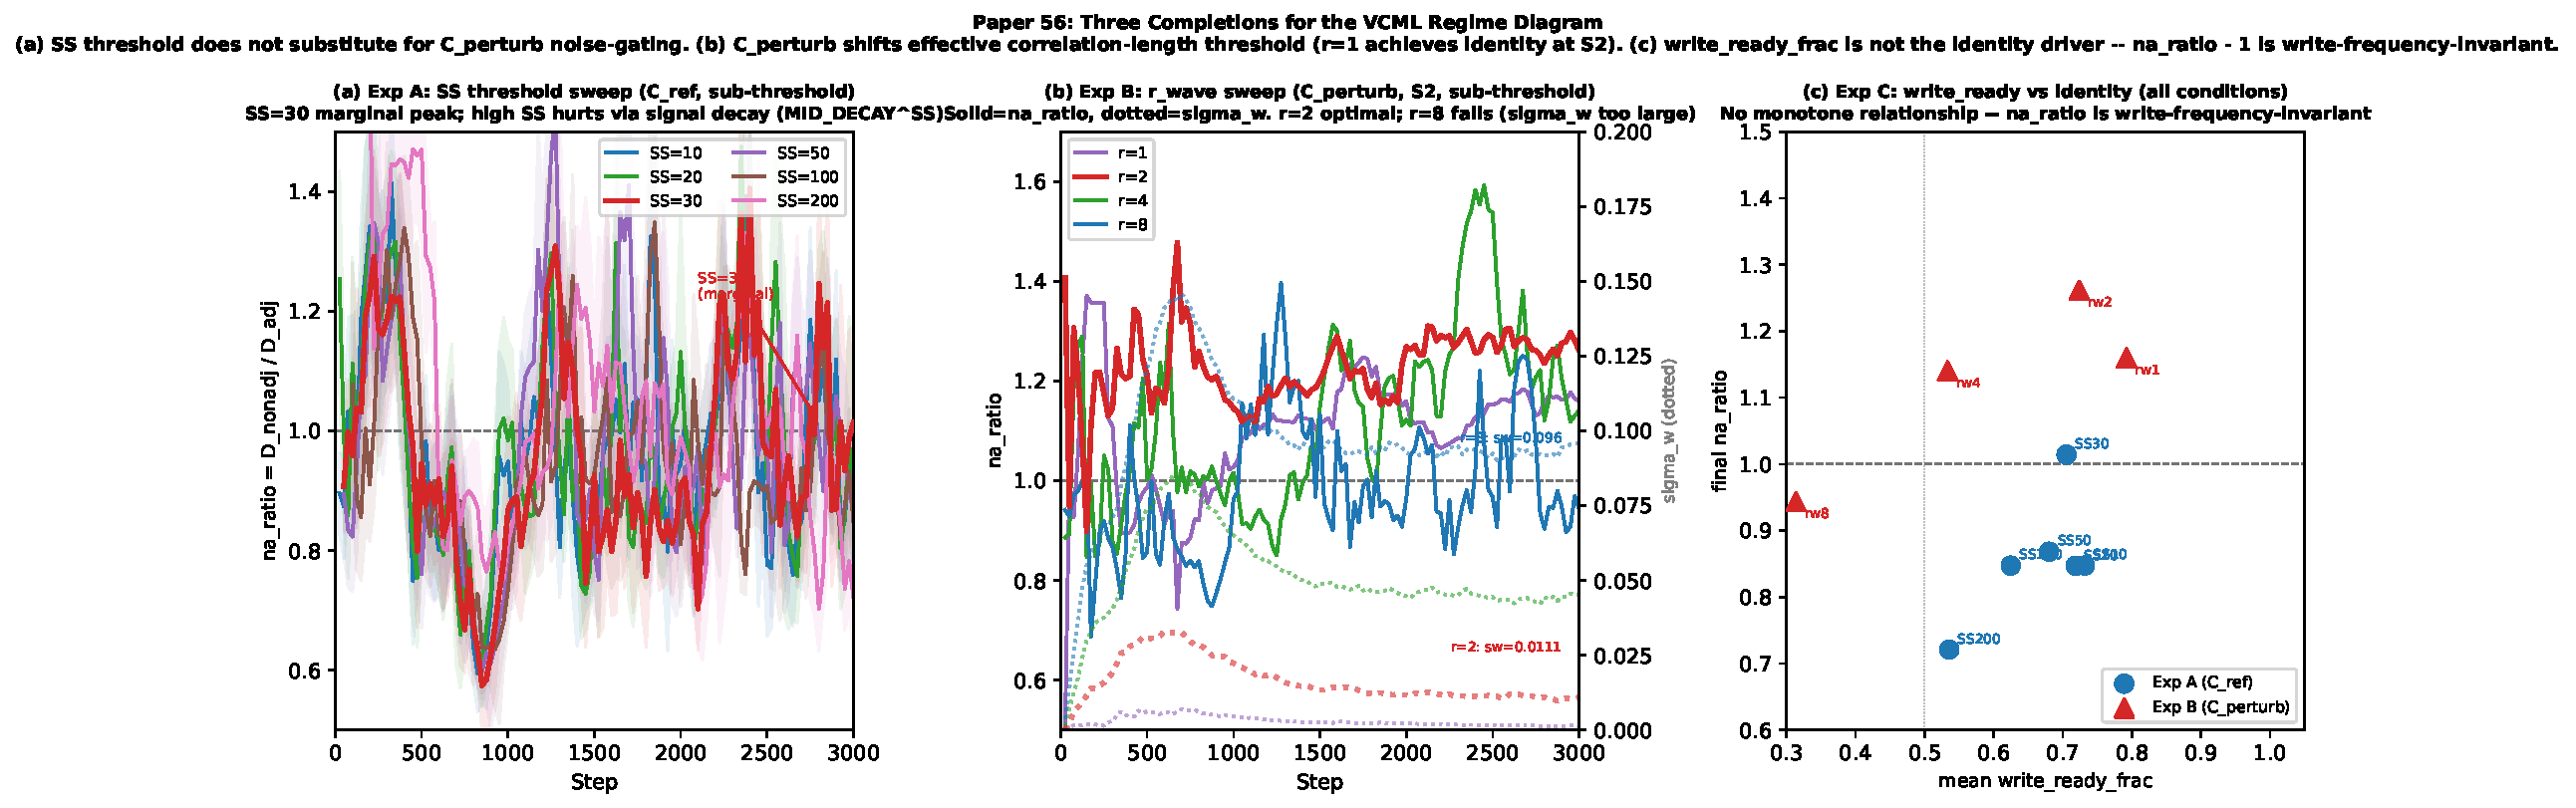
\includegraphics[width=\linewidth]{paper56_figure1.pdf}
  \caption{Three-panel figure. (a) Exp~A: na\_ratio($t$) for SS sweep.
    SS$=30$ (red) barely crosses identity threshold; higher SS regresses.
    (b) Exp~B: na\_ratio($t$) and $\sw$ (dotted) for $r_\mathrm{wave}$ sweep
    under C\_perturb at S2. $r=2$ optimal. Dotted lines illustrate noise-floor
    divergence at $r=8$.
    (c) Exp~C: scatter of write\_ready\_frac vs.\ final $\na$ for all conditions.
    No monotone trend; C\_perturb (triangles) achieves identity across the full
    write-frequency range.}
  \label{fig:main}
\end{figure}

\end{document}
